\documentclass[tikz, border=10pt]{standalone}
\usetikzlibrary{shapes.geometric, arrows.meta, positioning, calc, shapes.multipart, backgrounds, shadows}

\begin{document}
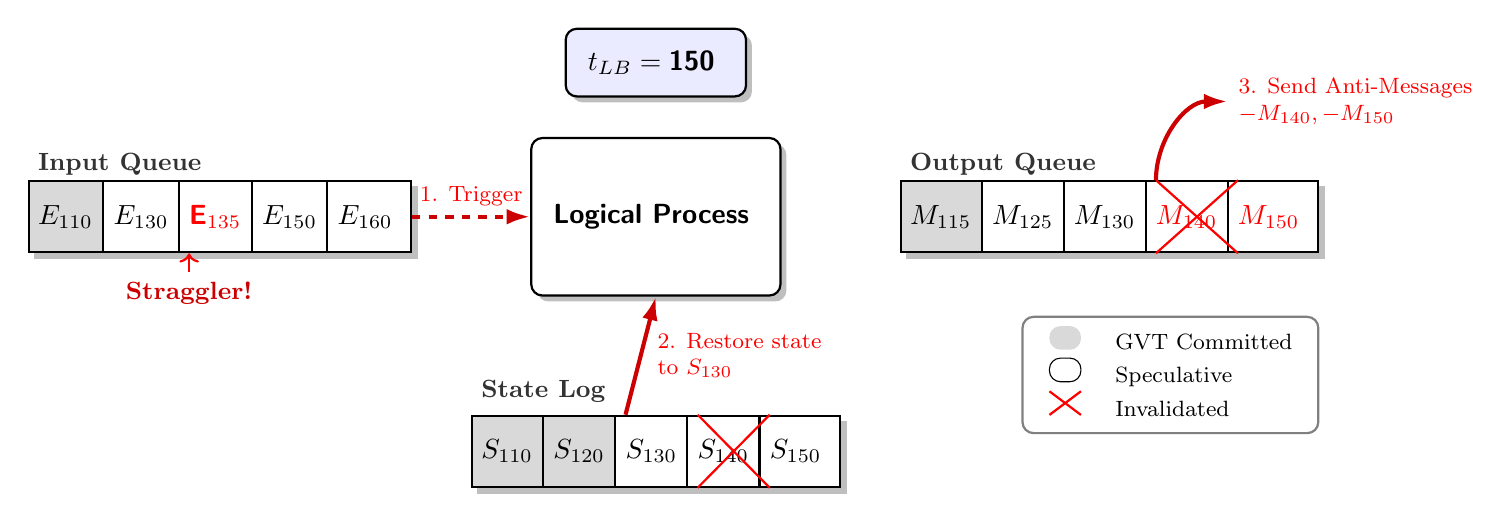
\begin{tikzpicture}[
    font=\sffamily,
    thick,
    component/.style={
        draw=black, 
        fill=white, 
        thick, 
        rounded corners,
        align=center,
        inner sep=8pt,
        drop shadow
    },
    queue/.style={
        draw=black,
        fill=none, 
        rectangle split, 
        rectangle split parts=5, 
        rectangle split horizontal=true,
        minimum height=0.9cm, 
        align=center
    },
    action arrow/.style={
        -{Latex[length=3mm, width=2mm]}, 
        line width=1.5pt,
        draw=red!80!black
    },
    label text/.style={
        font=\bfseries\small,
        color=gray!40!black
    }
]

    % Simulation Logic
    \node[component, minimum width=3cm, minimum height=2cm] (logic) at (0,0) {
        \textbf{Logical Process}
    };

    % Local Clock
    \node[component, fill=blue!8, above=0.5cm of logic] (lvt) {
        $t_{LB} = \textbf{150}$
    };

    % --- A. INPUT QUEUE (Left) ---
    \node[queue, left=1.5cm of logic, anchor=east] (inqueue) {
        \nodepart{one} $E_{110}$
        \nodepart{two} $E_{130}$
        \nodepart{three} $\textbf{\textcolor{red}{E}}_{\textcolor{red}{135}}$
        \nodepart{four} $E_{150}$
        \nodepart{five} $E_{160}$
    };
    \node[label text, above=0.2cm of inqueue.north west, anchor=west] {Input Queue};

    % --- B. OUTPUT QUEUE (Right) ---
    \node[queue, right=1.5cm of logic, anchor=west] (outqueue) {
        \nodepart{one} $M_{115}$
        \nodepart{two} $M_{125}$
        \nodepart{three} $M_{130}$
        \nodepart{four} \textbf{\textcolor{red}{$M_{140}$}}
        \nodepart{five} \textbf{\textcolor{red}{$M_{150}$}}
    };
    \node[label text, above=0.2cm of outqueue.north west, anchor=west] {Output Queue};

    % --- C. STATE LOG (Bottom) ---
    \node[queue, below=1.5cm of logic] (statequeue) {
        \nodepart{one} $S_{110}$
        \nodepart{two} $S_{120}$
        \nodepart{three} $S_{130}$
        \nodepart{four} $S_{140}$
        \nodepart{five} $S_{150}$
    };
    \node[label text, above=0.3cm of statequeue.north west, anchor=west] {State Log};

    % STRAGGLER & ROLLBACK ARROWS
    % --- Straggler Arrival ---
    \node[below=0.6cm of inqueue.three, text=red!80!black, font=\bfseries\small] (straggler_lbl) {Straggler!};
    \draw[->, red, thick] (straggler_lbl) -- (inqueue.three |- inqueue.south);

    % --- 1. Trigger ---
    \draw[action arrow, dashed] (inqueue.east) -- (logic.west) 
        node[midway, above, text=red, font=\footnotesize] {1. Trigger};

    % --- 2. Restore ---
    \draw[action arrow] (statequeue.three |- statequeue.north) -- (logic.south) 
        node[midway, right, text=red, font=\footnotesize, align=left, xshift=2pt] {2. Restore state\\ to $S_{130}$};

    % Cross out invalidated STATES
    \draw[red, thick] (statequeue.four |- statequeue.north) -- (statequeue.five |- statequeue.south);
    \draw[red, thick] (statequeue.four |- statequeue.south) -- (statequeue.five |- statequeue.north);

    % --- 3. Anti-Messages ---
    \draw[action arrow] (outqueue.four |- outqueue.north) to[out=90, in=180] 
        node[pos=1.0, right, text=red, align=left, font=\footnotesize] {3. Send Anti-Messages\\$-M_{140}, -M_{150}$} 
        ($(outqueue.north) + (1.5, 1.0)$);

    \draw[red, thick] (outqueue.four |- outqueue.north) -- (outqueue.five |- outqueue.south);
    \draw[red, thick] (outqueue.four |- outqueue.south) -- (outqueue.five |- outqueue.north);


    \begin{scope}[on background layer]
        \colorlet{gvtgray}{gray!30}

        \fill[white, drop shadow] (inqueue.north west) rectangle (inqueue.south east);
        \fill[gvtgray] (inqueue.north west) rectangle (inqueue.one split |- inqueue.south);

        \fill[white, drop shadow] (outqueue.north west) rectangle (outqueue.south east);
        \fill[gvtgray] (outqueue.north west) rectangle (outqueue.one split |- outqueue.south);

        \fill[white, drop shadow] (statequeue.north west) rectangle (statequeue.south east);
        \fill[gvtgray] (statequeue.north west) rectangle (statequeue.two split |- statequeue.south);

    \end{scope}

    % --- LEGEND ---
    \node[draw=gray, rounded corners, fill=white, anchor=north east, font=\footnotesize] 
        at ($(outqueue.south east) + (0, -0.8)$) {
        \begin{tabular}{c l}
            \tikz\fill[gray!30] (0,0) rectangle (0.4,0.3); & GVT Committed \\
            \tikz\fill[white, draw=black] (0,0) rectangle (0.4,0.3); & Speculative \\
            \tikz\draw[red, thick] (0,0) -- (0.4,0.3) (0,0.3) -- (0.4,0); & Invalidated
        \end{tabular}
    };

\end{tikzpicture}
\end{document}
